\documentclass[a4paper,11pt]{article}

%%%%%%%%%%%%%%%%%%%%%%%%%%%%%%%%%%%%%
% STD PACKAGES
%%%%%%%%%%%%%%%%%%%%%%%%%%%%%%%%%%%%%

\usepackage{amsthm,amsmath,amssymb,amsfonts}
\usepackage{marginnote}
\usepackage{enumerate}
\usepackage[colorlinks,citecolor=red]{hyperref}

\usepackage{subfigure}


%%%%%%%%%%%%%%%%%%%%%%%%%%%%%%%%%%%%%
% TIKZ
%%%%%%%%%%%%%%%%%%%%%%%%%%%%%%%%%%%%%

\usepackage{tkz-euclide}
\usetikzlibrary{patterns}
\usetikzlibrary{calc}
\usetikzlibrary{positioning}
\usetikzlibrary{decorations.pathmorphing}
\tikzstyle{point}=[draw,circle,fill=black,scale=.3] %draws a point call as \coordinate[point]
\tikzset{baseline={([yshift=-.5ex]current bounding box.center)}, every picture}

%%%%%%%%%%%%%%%%%%%%%%%%%%%%%%%%%%%%%
% THEOREMS
%%%%%%%%%%%%%%%%%%%%%%%%%%%%%%%%%%%%%

\theoremstyle{definition}
\newtheorem{remark}{Remark}

%%%%%%%%%%%%%%%%%%%%%%%%%%%%%%%%%%%%%
% CUSTOM COMMANDS
%%%%%%%%%%%%%%%%%%%%%%%%%%%%%%%%%%%%%

\makeatletter
\newcommand*{\defeq}{\mathrel{\rlap{%
    \raisebox{0.3ex}{$\m@th\cdot$}}%
  \raisebox{-0.3ex}{$\m@th\cdot$}}%
=}
\makeatother

\newcommand{\hooklongrightarrow}{\lhook\joinrel\longrightarrow}
\newcommand{\hooklongleftarrow}{\longleftarrow\joinrel\rhook}


\newcommand{\NN}{\mathbb{N}}
\newcommand{\ZZ}{\mathbb{Z}}
\newcommand{\QQ}{\mathbb{Q}}
\newcommand{\RR}{\mathbb{R}}
\newcommand{\CC}{\mathbb{C}}
\newcommand{\CP}{\mathbb{CP}}
\newcommand{\HH}{\mathbb{H}}
\newcommand{\DD}{\mathbb{D}}
\newcommand{\RP}{\mathbb{RP}}

\DeclareMathOperator{\GL}{GL}
\DeclareMathOperator{\SL}{SL}
\DeclareMathOperator{\PSL}{PSL}
\DeclareMathOperator{\SO}{SO}
\DeclareMathOperator{\SU}{SU}
\DeclareMathOperator{\PSU}{PSU}
\DeclareMathOperator{\U}{U}

\newcommand{\del}{\partial}
\newcommand{\delbar}{\bar{\partial}}
\newcommand{\F}{\mathcal{F}}
\newcommand{\OO}{\mathcal O}
\newcommand{\M}{\mathcal{M}}
\newcommand{\EE}{\mathcal{E}}
\newcommand{\Tr}{\mathrm{Tr}\,}
\renewcommand{\Im}{\mathrm{Im}}
\renewcommand{\Re}{\mathrm{Re}}

\newcommand{\mat}[4]{\begin{pmatrix} #1 & #2 \\ #3 & #4 \end{pmatrix}}
\newcommand{\vek}[2]{\begin{pmatrix} #1 \\ #2 \end{pmatrix}}


\usepackage{showlabels}

\title{Working Title}
\author{}
\date{\today}

\begin{document}

\maketitle

\tableofcontents

\section{Toy model: \texorpdfstring{$0d$ GLSM}{0d GLSM}}
\subsection{Setup}
We start with a $0d$ GLSM toy model, i.e.\ we consider the source manifold $\Sigma = \{ pt \}$ to be an abstract point and the target manifold to be $$X = \CP^{N-1} \times \CP^{N-1}$$
The space of fields is then simply given by points on the target manifold $X$, namely 
\begin{equation}
  \F = \CP^{N-1} \times \CP^{N-1}
\end{equation}
As the action of the model we consider 
\begin{equation}
  S(z,w) = \beta \lvert \langle \bar z, w\rangle \rvert^2 = \beta \sum_{j,k = 0}^{N-1} \bar z_j z_k \bar w_j w_k 
  \label{eq:toy_S}
\end{equation}
where $z,w \in \CC^{N}$ subject to the condition 
\begin{equation}
  \lvert z \rvert^2 = \sum_j \lvert z_j \rvert^2 = 1 \quad , \quad \lvert w \rvert^2 = \sum_k \lvert w_k \rvert^2 = 1
  \label{eq:toy_constr}
\end{equation}
The action enjoys a $\U(1) \times \U(1)$ gauge freedom (which here is simply a global $\U(1) \times \U(1)$ symmetry, acting as 
\begin{equation}
  e^{i\theta}\times e^{i\varphi}\colon (z,w) \mapsto (e^{i\theta} z, e^{i\varphi} w)
\end{equation}
Under the assumption of the condition \eqref{eq:toy_constr}, the action \eqref{eq:toy_S} does define a function on $\CP^{N-1} \times \CP^{N-1}$.

The path integral of the model is defined by 
\begin{equation}
  Z = \int \prod_j dz_j d\bar z_j dw_j d\bar w_j \delta(\lvert z \rvert^2  - 1)\delta(\lvert w \rvert -1)  e^{-S(z,w)}
  \label{eq:toy_Z}
\end{equation}
In order to evaluate \eqref{eq:toy_Z}, we want to embed the space of fields $\mathcal F = \CP^{N-1} \times \CP^{N-1}$ into a higher dimensional complex space such that 
\begin{enumerate}
  \item the new action $\tilde S$ is holomorphic in the new variables (fields)
  \item when we restrict to $\mathcal F$, $\tilde S$ reduces to $S$
\end{enumerate}
We think of this embedding as an analytic continuation of the space of fields in an appropriate sense.

\subsection{Complexification of Real Analytic Manifolds}
Let us first recall a basic construction of complexification of real analytic manifolds due to Bruhat and Whitney \cite{Bruhat_Whitney}.

Let $M$ be a real analytic manifold of dimension $\dim_{\RR} M = m$.
Moreover, let $\{ U_i, \phi_i \}$ be a real analytic atlas of $M$, with $U_i \subset \RR^m$ and charts $\phi_i \colon U_i \to M$ so that the transition functions
\begin{equation}
  \phi_{ij} = \phi_j^{-1} \circ \phi_i \colon U_{ij} \to U_{ij}
\end{equation}
are real analytic diffeomorphisms.
The idea of complexifying $M$ is to find a complex manifold $M^{\CC}$ with $\dim_{\CC} M^{\CC} = m$ and a (real analytic) isomorphism $f\colon M \to \tilde M \subset M^{\CC}$ of $M$ onto a submanifold of $M^{\CC}$. 
(Fancy way to say that $M$ should be a real analytic submanifold of $M^{\CC}$ up to isomorphism)
Now, find opens $U_i^{\CC} \subset \CC^m$ such that $U_i^{\CC} \cap \RR^m = U_i$ and extend the charts $\phi_i$ charts $\phi_i^{\CC}$ such that 
\begin{enumerate}[(i)]
  \item the transition functions $\phi^{\CC}_{ij} \colon U^{\CC}_{ij} \to U^{\CC}_{ij}$ are biholomorphic

  \item $\phi^{\CC}_{ji} = \left( \phi^{\CC}_{ij} \right)^{-1}$ and $\phi^{\CC}_{ii} = id$

  \item the transition functions $\phi^{\CC}_{ij}$ satisfy the usual 2-cocycle condition (gluing condition) on $U^{\CC}_{ijk}$: $\phi^{\CC}_{ij}\circ\phi^{\CC}_{jk} = \phi^{\CC}_{ik}$
\end{enumerate}
These conditions ensure that we can glue $M^{\CC}$ from the local data $\{ U_i^{\CC}, \phi_i^{\CC} \}$:
\begin{equation}
  M^{\CC} = \coprod_i U_i^{\CC} / \sim \quad , \quad z_i \sim z_j \text{~iff~} z_j = \phi^{\CC}_{ji}(z_i) \text{~on~} U^{\CC}_{ij}
\end{equation}

For more details on this construction see \href{https://books.google.ca/books?id=In1Dbj-pkIkC&pg=PA103\&dq=complexification+of+real+analytic+manifolds\&hl=en&sa=X\&ei=aYRAUrWeBYPZ2AWEj4DoBA\&ved=0CD8Q6AEwAQ#v=onepage\&q=complexification\%20of\%20real\%20analytic\%20manifolds&f=false}{Cieliebak and Eliashberga's book} \cite{CEbook}

\subsubsection{Example: The \texorpdfstring{$N$-sphere}{N-sphere}}
Consider the $N$-sphere $S^{N} \subset \RR^{N+1}$.
First, consider the following atlas: let $p_{\pm} = (0, \dots,0, \pm 1) \in S^{N}$ be the north and south pole respectively.
We denote points on the sphere by $x = (x_1, \dots, x_{N+1})$, $\lVert x \rVert^2 = 1$ and points in $\RR^N$ by $X = (X_1, \dots, X_N)$.
The atlas we consider is given by steoreographic projection through $p_{\pm}$:
Let $U_{\pm} = \RR^N$ and $V_{\pm} = S^N - \{ p_{\pm} \}$. 
Then define charts
\begin{equation}
  \phi_{\pm} \colon U_{\pm} \to V_{\pm} \subset S^N \quad , \quad X \mapsto \left( \frac{2 X}{1 + \lVert X \rVert^2}, \pm \frac{\lVert X \rVert^2 - 1}{\lVert X \rVert^2 + 1} \right)
\end{equation}
with inverse
\begin{equation}
  \phi_{\pm}^{-1} \colon x \mapsto \left\{\frac{x_i}{1 \mp x_{N+1}}\right\}
\end{equation}
From this, one finds the transition functions
\begin{equation}
  \phi_{+-} = (\phi_{-+})^{-1} = \phi_{-}^{-1}\circ \phi_{+} \colon X \mapsto \frac{X}{\lVert X \rVert^2}
\end{equation}
\begin{remark}
  There is a nice geometric interpretation of these transition functions.
  Note that the map 
  \begin{equation}
    X \mapsto \frac{X}{\lVert X \rVert^2}
  \end{equation}
  describes an involution at the unit sphere $S^{N-1}$.
  On the sphere, the maps differ merely by a sign switch in the $x_{N+1}$ component and indeed, if one computes the transition functions directly on the embedded sphere (that is as maps from $\RR^{N+1} \to \RR^{N+1}$) one finds
  \begin{equation}
    \phi_{+} \circ \phi_{-} \colon (x_i, x_{N+1}) \mapsto (x_i, - x_{N+1})
  \end{equation}
  which corresponds to a reflection of $x$ about the equator! (It helps visualising this for the case 2-sphere)
  But under stereographic projection, a reflection about the equator becomes an inversion on the unit sphere $S^{N-1}$ in $\RR^N$ (again, it helps working this out in the case $N=2$).
\end{remark}

Now, since $U_{\pm} = \RR^N$ there exist obvious candidates for a complexification, namely $U^{\CC}_{\pm} = \CC^N$. 
We thus promote every $X$ to a complex variable $Z = X + i Y$.
Conversely, we can promote any $x \in \RR^{N+1}$ satisfying $\lVert x \rVert^2 = \sum_j x_j^2 = 1$ to complex variables $z$ satisfying 
\begin{equation}
  \sum_j z_j^2 = 1
  \label{eq:toy_quadric}
\end{equation}
The above equation defines a hypersurface (so-called \emph{quadric}) inside $\CC^{N+1}$.

There is a very interesting observation I found in \href{https://math.stackexchange.com/questions/1784898/tangent-bundle-of-sphere-as-a-complex-manifold}{this} stackexchange post: the quadric $Q$ defined by \eqref{eq:toy_quadric} is \emph{diffeomorphic} to the tangent space $TS^N$.
The diffeomorphism is realised by the following map:
\begin{equation}
  \Psi \colon TS^{N} \to Q \quad , \quad (x,y) \mapsto z = \Psi(x,y) = x \sqrt{1 + \lVert y \rVert^2} + i y
\end{equation}
with inverse 
\begin{equation}
  \Psi^{-1}(x + i y) = \left( \frac{x}{\sqrt{1 + \lVert y \rVert^2}}, y \right) 
\end{equation}
where $\lVert y \rVert^2 = \sum_{i} y_i^2$.
\begin{remark}
Verification that $\Psi$ does indeed define a diffeomorphism goes by a straight forward calculation.
(Recall in particular that the tangent space $TS^N$ can be described by pairs $(x,y) \in \RR^{N+1}$ such that $\langle x, y\rangle = \sum_i x_i y_i = 0$)
\end{remark}

There exists another very interesting diffeomorphism (which I have discovered in this \href{https://math.stackexchange.com/questions/4871752/tangent-bundle-of-a-sphere-t-mathbb-sn-is-diffeomorphic-to-mathbb-sn-time}{stackexchange post}
\begin{equation}
  \Phi \colon S^N \time S^N / \Delta \to TS^N \quad , \quad (u,v) \mapsto \left( u, \frac{v - \left\langle u, v \right\rangle u}{1 - \left\langle u, v \right\rangle } \right)
  \label{eq:diff_SNSN_TSN}
\end{equation}
Its inverse is given by 
\begin{equation}
  \Phi^{-1} \colon TS^N \to S^N \times S^N / \Delta \quad , \quad (x,y) \mapsto \left( x, \frac{x(\lVert y \rVert^2 - 1) + 2 y}{\lVert y \rVert^2 + 1} \right)
\end{equation}
\begin{remark}
  The map \eqref{eq:diff_SNSN_TSN} is the sterepgraphic projection of $v \in S^N$ through the ``pole'' $u \in S^N$.
\end{remark}
Finally we have the following commutative diagram 
\begin{equation}
  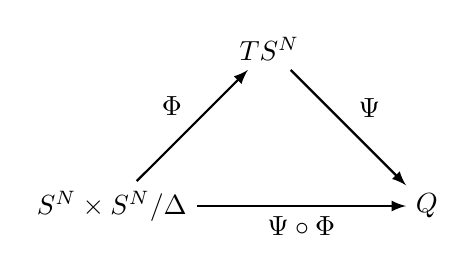
\begin{tikzpicture}
    \node (TS) at (0,2) {$TS^N$};
    \node (SS) at (-2,0) {$S^N \times S^N / \Delta$};
    \node (Q) at (2,0) {$Q$};

    \draw[thick,-{latex}] (SS) -- node[midway,below] {$\Psi\circ\Phi$}(Q);
    \draw[thick,-{latex}] (TS) -- node[midway, above right] {$\Psi$} (Q);
    \draw[thick,-{latex}] (SS) -- node[midway, above left] {$\Phi$} (TS);
  \end{tikzpicture}
\end{equation}

The idea is that we can use $S^N \times S^N$ to parametrise $Q$ nicely and that maybe the action of $\U(1)$ on $S^N$ can naturally be lifted to a diagonal action on $S^N \times S^N$.
In fact, I believe that the $\U(1)$ action on $S^N$ leaves the norm in variant sp that the map $\Psi \circ \Phi$ has a chance to be an equivariant map. 
However, this remains to be checked!


\begin{thebibliography}{99}
  \bibitem{Bruhat_Whitney} F.\ Bruhat and H.\ Whitney, Quelques propri\'et\'es fondamentales des ensembles analytiques-r\'eels, Comment. Math. Helv. 33, 132-160 (1959).

  \bibitem{CEbook} K.\ Cieliebak and Y.\ Eliashberg. From Stein to Weinstein and back: symplectic geometry of affine complex manifolds. Vol. 59. American Mathematical Soc., 2012.
\end{thebibliography}
\end{document}
